\subsection{了解神经网络}
如今神经网络在各个领域都有涉及, 在计算机视觉领域更是有极大的优越性。从机器学习再到深度学习,几乎已经形成一个完整的
技术体系并且仍然在高速发展。
通常来说,神经网络一般有以下三个作用:
\begin{enumerate}
    \item \textbf{预测}: 这通常是一维层面的,通过给予计算机一定量已有的数据(通常是多组自变量和因变量)拟合出一个合适的曲线(函数),当有新的自变量传入的时候,通过该曲线给出预测的结果
    \item \textbf{识别}: 这通常是二维层面的,同样是给予计算机一定量的二维图像,同时告诉计算机我们想要识别的图像主体,给予其标注,通过大量数据的学习让计算机能够准确识别任意图像中符合要求的部分
    \item \textbf{自然语言}: 通过给予海量的文本数据,使计算机能够理解、解释和生成自然语言,进行情感分析和语言推断。
\end{enumerate}
这些只是对作用的简单解释,具体过程要比这复杂的多。

无论是一维的预测还是二维的识别,从本质上来说,所谓\textbf{学习},就是不断调整神经网络内部参数使参数达到一种足够泛化也足够准确的大小,能够保证传入
的数据在经过这群参数组成的\textbf{“函数"}映射后,得到一个可信度高的答案。
那么在拟合这群参数后,如果没有处理好,会出现\textbf{欠拟合}和\textbf{过拟合}的问题

\begin{figure}[h]
    \centering
    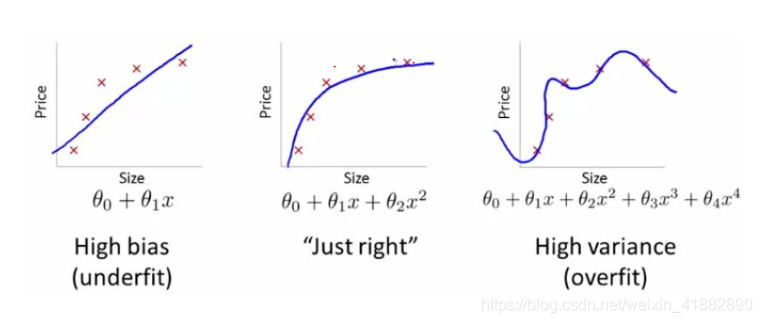
\includegraphics[width=0.8\textwidth]{拟合.png}
    \caption{欠拟合与过拟合}
    \label{fig:拟合}
\end{figure}

如图所示,欠拟合就是参数调整的太差了,根本没有预测的能力,得到的答案和实际上差距非常大,这时候我们就应该考虑增加训练数据或者
是增强数据的特征。

另一个过拟合,就是数据的特征过于明显或者是训练的过强导致网络没有足够的泛化能力,那么当传入的数据不是训练的数据的时候,将无法正确
预测,这时候就应该减少训练的次数,减少数据集的数量或者是降低数据的特征,提高泛化能力,

通过简单的了解,我们知道神经网络的作用以及神经网络是如何训练出来的,现在我们将通过自己动手搭建一个神经网络,在学习搭建的过程中对
更深入的内容进行讲述。
\subsection{动手搭建神经网络}
如果我们的网络只有简单的功能需求,那么用当今主流的pytorch就可以快速构建起一个神经网络,pytorch中封装好了很多搭建网络所需要的功能
我们只需要简单理解就能够直接调用使用。如果我们对准确性,效率等有更高的要求,可以使用已有的框架比如yolo,只需要准备好数据集和标注,按照需求
简单调整一下框架的参数,就可以训练出一个高性能的网络。

我们将从安装开始,一步步利用\textbf{pytorch}搭建出一个简单的识别图像中数字的网络。
\subsubsection{虚拟环境——Anaconda}
在安装Pytorch之前,我们要先安装Anaconda。

什么是Anaconda?一般来说在电脑上已经安装好了一个python环境,但是对于不同的项目需要不同的python环境
同时这些项目还要安装各种包和依赖,如果都把他们放在我们电脑最基础的环境下,很容易出现各种冲突问题而且很难管理。Anaconda能为我们创建不同的虚拟环境,
我们可以按照需要在这些虚拟环境里安装不同的包和依赖,它们不会相互影响,而且不同环境之间相互切换,操作简单,非常方便。同时Anaconda还有超过180个科学包和
依赖项,简单的几行命令就可以将这些包安装到指定的虚拟环境下,省去了麻烦的下载流程和令人头疼的配置过程。我们将用Anaconda创建一个独属于pytorch的虚拟环境。

Anaconda官方下载地址:\url{https://www.anaconda.com/download/}

按照官方流程安装好Anaconda后,在Windows的Anaconda Prompt(ubuntu的终端)输入
\begin{tbash}
    conda --version
\end{tbash}
如果显示版本号,说明安装成功。

\textbf{创建虚拟环境}

在Anaconda Prompt输入
\begin{tbash}
    conda create -n pytorch python=3.7
\end{tbash}
这样我们就创建了一个名为pytorch的虚拟环境,同时指定了python的版本为3.7,这样我们就可以在这个环境下安装pytorch了。

\textbf{激活虚拟环境}

在Anaconda Prompt输入
\begin{tbash}
    conda activate pytorch
\end{tbash}
我们会发现命令行前面多了(pytorch)字样,这就说明我们已经成功激活了pytorch环境。
这时输入
\begin{tbash}
    pip list
\end{tbash}
就可以看到当前环境下已经安装的包。
类似的
\begin{tbash}
    conda deactivate
\end{tbash}
就退出了当前环境。

\subsubsection{安装Pytorch}
在激活了pytorch环境后,我们就可以安装pytorch了。
在命令行输入
\begin{tbash}
    pip install pytorch torchvision
\end{tbash}
这样我们就安装好了pytorch,同时还安装了torchvision这个包是pytorch的辅助包,用于处理图像。
\textit{如果你出现了诸如网络问题导致无法安装,请改变虚拟环境的源为国内源,具体操作请自行搜索}

这样我们就安装好了pytorch-CPU,如果你有NVIDIA的显卡,可以考虑安装pytorch-GPU,网络的训练速度和推理速度会更快。
可以在命令行输入
\begin{tbash}
    nvidia-smi
\end{tbash}
查看自己的显卡型号,然后在官网上查看对应的CUDA版本,再安装对应的pytorch-GPU版本。
这里给上CUDA的官网下载地址:\url{https://developer.nvidia.com/cuda-toolkit-archive}
刚刚的pip install命令可以改为
\begin{tbash}
    pip3 install torch torchvision torchaudio --index-url https://download.pytorch.org/whl/cu{你的CUDA版本}
\end{tbash}

\subsubsection{搭建神经网络}
接下来用pytorch搭建一个简单的LeNet网络,识别MNIST数据集中的手写数字

选择一个你喜欢的IDE,比如VSCode, Pycharm, Clion等,创建一个python文件,选择解释器为刚刚创建的虚拟环境。
如果你感觉IDE的配置比较麻烦,也可以试试jupyter notebook,它是一个交互式的笔记本,可以直接在浏览器上运行代码,适合学习使用。

准备好后,首先导入需要的包
\begin{tpython}
    import torch
    import torch.nn as nn
    import torch.optim as optim
    import torchvision
    import torchvision.transforms as transforms
    import matplotlib.pyplot as plt
\end{tpython}
\begin{enumerate}
    \item torch: pytorch的核心包,包含pytorch的核心数据结构,以及所有的操作
    \item torch.nn: pytorch的神经网络包,包含所需的神经网络模块。
    \item torch.optim: pytorch的优化器包,包含了所有的优化器。
    \item torchvision: pytorch的图像处理包,包含了图像处理的所有操作。
    \item torchvision.transforms: pytorch的图像变换包,包含了所有的图像变换操作。
    \item matplotlib.pyplot: 画图的包,我们用来画出训练过程中的一些曲线。
\end{enumerate}

接下来准备MINST数据集

MINST数据集是一个包含了6万张训练图片和1万张测试图片的数据集,每张图片都是各式各样的手写的数组,每张图片上都有一个0-9的数字标签。
我们可以通过torchvision包中的datasets来下载这个数据集。
\begin{tpython}
    train_dataset = torchvision.datasets.MNIST(root='./data', train=True, transform=transforms.ToTensor(), download=True)
    test_dataset = torchvision.datasets.MNIST(root='./data', train=False, transform=transforms.ToTensor(), download=True)
\end{tpython}
这里的参数含义分别是:
\begin{enumerate}
    \item root: 数据集的存放路径
    \item train: 是否是训练集,True表示训练集,False表示测试集
    \item transform: 数据集的变换方式,这里是ToTensor(),将图片转换为tensor张量
    \item download: 是否下载数据集,如果已经下载过了,可以设为False
\end{enumerate}

但这里我们需要对数据集进行更多的转变操作,利用Compose将多个变换组合在一起,比如ToTensor()转化成Tensor和Normalize归一化
\begin{tpython}
    compose=torchvision.transforms.Compose([
        torchvision.transforms.ToTensor(),
        torchvision.transforms.Normalize((0.1307,), (0.3081,))
    ])

    train_dataset = torchvision.datasets.MNIST(root='./data', train=True, transform=compose, download=True)
    test_dataset = torchvision.datasets.MNIST(root='./data', train=False, transform=compose, download=True)
\end{tpython}

然后通过DataLoader加载数据集,使我们可以迭代访问数据集
\begin{tpython}
    train_loader = torch.utils.data.DataLoader(dataset=train_dataset, batch_size=64, shuffle=True)
    test_loader = torch.utils.data.DataLoader(dataset=test_dataset, batch_size=64, shuffle=False)
\end{tpython}
这里的参数含义分别是:
\begin{enumerate}
    \item dataset: 加载的数据集
    \item batch\_size: 一次加载的数据量, 这里是$64$
    \item shuffle: 是否打乱数据集
\end{enumerate}

我们完成了对数据集的准备,接下来搭建最基础最经典的LeNet网络结构:
\begin{figure}[H]
    \centering
    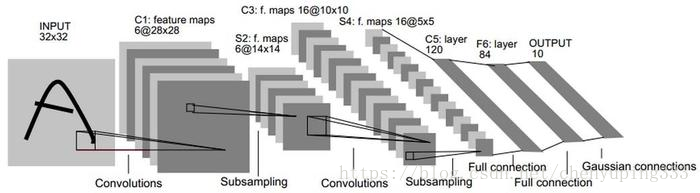
\includegraphics[width=0.7\textwidth]{images/LeNet.png}
    \caption{LeNet网络结构}
    \label{fig:LeNet}
\end{figure}

可以看到,除去输入层,LeNet一共有7层,按顺序进行卷积,池化,卷积,池化,全连接,全连接,全连接操作。

我们先对卷积,池化操作进行解释。

\textbf{卷积操作}:

卷积操作是神经网络中基本也是重要的操作之一,目的是提取图像的特征,通过一个n*n的卷积核在图像上滑动,将卷积核中心的像素大小替换为该卷积核上所有像素大小的加权和
\begin{figure}[H]
    \centering
    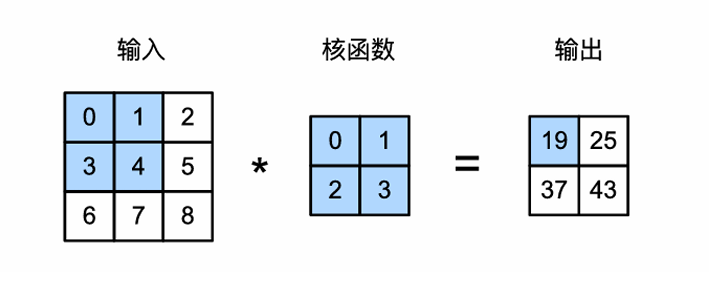
\includegraphics[width=0.7\textwidth]{images/卷积.png}
    \caption{卷积操作}
    \label{fig:卷积}
\end{figure}
用公式表示为:
\begin{equation}
    [H]_{i,j}=\sum_{a=-\Delta }^{\Delta}\sum_{b=-\Delta}^{\Delta}[V]_{a,b}[X]{i+a,j+b}   
\end{equation}
其中$[H]$是卷积后的图像,$[V]$是卷积核,$[X]$是原图像,$\Delta$是卷积核的大小。
这就是一次卷积层的操作。

我们要根据需要调整卷积核的大小,填充,步幅等参数。
\begin{enumerate}
    \item 卷积核大小: 通常是一个奇数,比如$3\times3$,$5\times5$,$7\times7$等
    \item 填充: 由于卷积核不是$1\times1$,所以边缘像素无法进行卷积,在多次卷积后,图像像素显著减少会失去许多信息,这就需要填充对图像进行扩充。
    \item 步幅: 卷积核每次滑动的步长,步长越大,卷积出的图像尺寸越小
\end{enumerate}
一般输出图像的形状为
\begin{equation}
    (n_{h}-k_{h}+p{h}+1) \times (n_{w}-k_{w}+p_{w}+1)
\end{equation}
其中$n_{h},n_{w}$是输入图像的高和宽,$k_{h},k_{w}$是卷积核的高和宽,$p_{h},p_{w}$是填充的高和宽。

\textbf{池化操作}:

池化操作是为了减少数据量,减少计算量,同时保留图像的主要特征,目的是减低卷积层对位置的敏感性。

汇聚层和卷积层相似,由一个池化核(池化窗口)在输入的信息上移动,同
样具有填充和步幅两个参数。汇聚操作计算的是窗口
中数据的最大值或者是平均值,这些操作分别称为\textbf{最大汇聚层}和\textbf{平均汇聚层}
\begin{figure}[H]
    \centering
    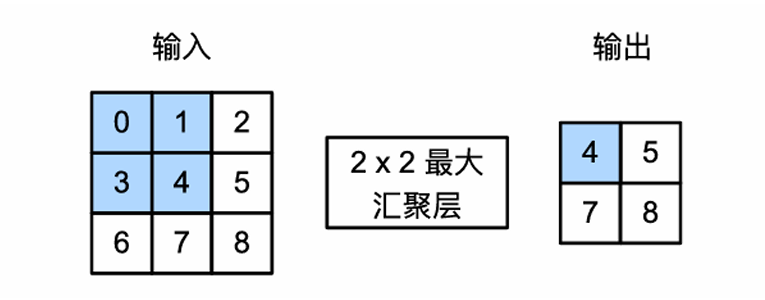
\includegraphics[width=0.7\textwidth]{images/池化.png}
    \caption{池化操作}
    \label{fig:池化}
\end{figure}

\textbf{全连接层}:

全连接层通常作为输出层使用,负责将网络的高层特征映射到最终的类别概率。
通常是为了整合特征,减少特征的维度,得到最终的输出类别。

\textbf{激活函数}:

这里我们涉及一下激活函数。
激活函数是神经网络中非常重要的一部分,它的作用是引入非线性因素,使得神经网络可以拟合任意复杂的函数。
通过加权和以及偏置来确定神经元是否应该激活,将输入信号转换为输出的
可微运算。大多数激活函数都是非线性的。
我们将主要用到ReLU激活函数,这是一个非常纯粹的函数:
\begin{equation}
    ReLU(x)=max(0,x)
\end{equation}
抛弃所有负元素,它求导表现得特别好:要么让参数消失,要么让参数通过

除此之外,还有sigmoid函数:
\begin{equation}
    sigmoid(x)=\frac{1}{1+\exp{-x}} 
\end{equation}
又称挤压函数,将($-\infty$,$\infty$)的任意数压缩到( $0$ , $1$ )

如此我们了解了神经网络的一些基本操作。

\textbf{搭建网络}:

首先写一个LeNet类,继承nn.Module
\begin{tpython}
    class LeNet(nn.Module):
        def __init__(self):
            super(LeNet, self).__init__()
            self.conv1=nn.Conv2d(1,6,5)
            self.pool1=nn.MaxPool2d(2,2)
            self.conv2=nn.Conv2d(6,16,5)
            self.pool2=nn.MaxPool2d(2,2)
            self.fc1=nn.Linear(16*5*5,120)
            self.fc2=nn.Linear(120,84)
            self.fc3=nn.Linear(84,10)
\end{tpython}

我们这里定义了LeNet类,并且在初始化函数中定义了一些层
显而易见
\textbf{卷积层}:
\begin{tpython}
    self.conv1=nn.Conv2d(3,16,5)
\end{tpython}
参数分别是\textbf{输入通道数,输出通道数,卷积核大小}。
我们知道图片是由RGB三个通道组成,因此这里输入通道数为3,按照LeNet的结构,让输出通道数为16,这是第一个卷积层。第二个卷积层同理,输入通道数为16,输出通道数为32。

\textbf{池化层}:
\begin{tpython}
    self.pool1=nn.MaxPool2d(2,2)
\end{tpython}
参数分别是\textbf{池化核大小,步幅}。
这里的池化核大小是2,步幅也是2,这是第一个池化层。第二个池化层同理。

\textbf{全连接层}:
\begin{tpython}
    self.fc1=nn.Linear(16*5*5,120)
\end{tpython}
参数分别是\textbf{输入特征数,输出特征数}。
输入特征数数根据上一层也就是池化层的输出决定。后面两个全连接层同理。
在最后一个全连接层我们输出10个特征,因为MNIST数据集中有10个类别(0 ~ 9)。

接下来我们定义前向传播函数,也就是网络的计算过程,处理输入数据,输出预测结果。
\begin{tpython}
    def forward(self, x):
        x=nn.relu(self.conv1(x))
        x=self.pool1(x)
        x=nn.relu(self.conv2(x))
        x=self.pool2(x)
        x=x.view(-1,16*5*5)
        x=nn.relu(self.fc1(x))
        x=nn.relu(self.fc2(x))
        x=self.fc3(x)
        return x
\end{tpython}
和上面的架构一样,只是在每次卷积操作后进行了激活操作,以及全连接层后进行了激活操作。
\textbf{x.view}:
这个函数是将一个多维的tensor转换为一维的tensor,参数-1表示自动计算,这里是将16*5*5的tensor转换为一维的tensor。
符合后面的全连接层输入。

如果想让网络每个处理更加简洁,可以使用\text{Sequential容器},将网络的层组合在一起。
比如我们可以将一次卷积,激活,池化操作组合在一起
\begin{tpython}
    self.conv1=nn.Sequential(
        nn.Conv2d(3,16,5),
        nn.ReLU(),
        nn.MaxPool2d(2,2)
    )
\end{tpython}
这样在forward函数中就可以直接调用这个容器,更加简洁。

这样我们就搭建好了一个简单的LeNet网络
\begin{tpython}
    Net=LeNet() 
\end{tpython}
实例化我们的网络

\textbf{定义损失函数:}

损失函数负责责量化实际值和预测值之间的差距,数值越小损失越小,因此我们通常要追求更小的损失。比如,平方误差函数
\begin{equation}
    l^{(i)}(\textbf{w},b)=\frac{1}{2}(\hat{y}^{(i)}-y^{(i)})^{2}
\end{equation}
$\hat{y}$表示预测值,$y$表示实际值,公式代表在$w$权重,$b$偏置下预测值和实际值的误差
一般情况下,我们要计算训练集上n个样本的平均损失L
\begin{equation}
    L(\textbf{w},b)=\frac{1}{n}\sum_{i=1}^{n}l^{(i)}(\textbf{w},b)
\end{equation}

在LeNet中我们使用\textbf{交叉熵损失函数}:
交叉熵公式:
\begin{equation}
    H(y,\hat{y})=-\sum_{i}y_{i}\log{\hat{y}_{i}}
\end{equation}
其中y是实际值,$\hat{y}$是预测值,交叉熵损失函数是一个非负函数,当预测值和实际值相等时,交叉熵为0,否则交叉熵越大,预测值和实际值差距越大。

代码中我们定义损失函数:
\begin{tpython}
    criterion=nn.CrossEntropyLoss()
\end{tpython}

\textbf{定义优化器:}

优化器负责更新网络的参数,使得损失函数最小化,这里我们使用\textbf{Adam优化器}:
Adam优化器是一种自适应学习率的优化器,它可以根据梯度的大小自动调整学习率,使得训练更加稳定。
所谓\textbf{学习率},就是每次更新参数的步长,学习率越大,参数更新的幅度越大,学习率越小,参数更新的幅度越小。
因此动态调整学习率有一定的重要性,降低梯度爆炸和梯度消失的风险。

\begin{tpython}
    optimizer=optim.Adam(Net.parameters(),lr=0.001)
\end{tpython}
这里的参数含义分别是\textbf{网络的参数,学习率}。Net.parameters()自带的函数,可以返回网络中所有的参数。

我们已经定义好了网络,损失函数,优化器,接下来我们就可以开始训练网络了。

\subsubsection{训练与测试网络}
在定义训练函数之前,我们需要了解一下网络训练过程中调整参数的主要方式——\textbf{反向传播}:

首先是\textbf{前向传播},前向传播是指从输入层到输出层的计算过程,通过输入数据,经过一系列的计算,得到输出结果。
这期间会储存一些中间变量,以便后续的反向传播。

反向传播是计算神经网络参数梯度的方法,该方法根据微积分中的\textbf{链式规则},按相反的
顺序从输出层到输入层遍历网络。该算法存储了计算某些参数梯度时所需的任何中间变量(偏导数)

在训练神经网络时,在初始化模型参数后,我们交替使用前向传播和反向传播,利用反向传播给出的梯度来更新模型参数。

\textit{反向传播需要利用前向传播中储存的中间值,因此我们一般需要保存这些中间值,这就导致需要更大的显存。
这些中间值的大小与网络层的数量和批量的大小大致成正比。
因此,使用更大的批量来训练更深层次的网络更容易导致\textbf{显存}不足(out of memory)错误}

就像前面所说的,神经网络训练本质上是调整参数,参数好坏的标准就是损失函数,我们要让损失函数尽可能的小,这其中用到了一个非常重要的算法——\textbf{梯度下降}:
梯度下降是一种优化算法,通过不断的往损失函数减小的方向上来更新参数以此降低误差,来达到优化模型的目的。
更新过程:
\begin{equation}
    (\textbf{w},b) \longleftarrow (\textbf{w},b) - \frac{\eta}{\left\lvert\mathcal{B}\right\rvert}\sum_{i\in\mathcal{B}}\partial_(\textbf{w},b)l^{(i)}(\textbf{w},b)
\end{equation}
\begin{enumerate}
    \item $\eta$: 学习率,控制参数更新的步长
    \item $\mathcal{B}$ : 批量大小,每次更新参数的样本数
    \item $\partial$ : 偏导数,迭代的是哪个参数就对哪个参数求偏导
    \item $l^{(i)}$ : 损失函数求得的损失
\end{enumerate}
这其中\textbf{学习率和批量}是手动设置的,是\textbf{超参数}。需要不断调整来达到最优效果。
在实际过程中,超参数的设置是十分关键的,这需要常年累月的调参经验。

\textit{算法只能使损失向最小值缓慢\textbf{收敛},无法在有限步数下准确求出最小值}

接下来我们定义train函数,用于训练网络
\begin{tpython}
    def train(epoch) # 传入当前的轮次
        running_loss=0.0 # 累加损失
        running_total=0 # 累加样本总数
        running_correct=0 # 累加正确样本数
        for batch_idx, data in enumerate(train_loader,0): # 遍历训练集
            inputs, labels=data # 获取输入和标签
            optimizer.zero_grad() # 梯度清零

            # forward + backward + optimize
            outputs=Net(inputs) # 前向传播
            loss=criterion(outputs,labels) # 计算损失
            loss.backward() # 反向传播
            optimizer.step() # 更新参数,优化

            running_loss+=loss.item() # 累加损失
            _, predicted=torch.max(outputs,dim=1) # 获取预测值
            running_total+=inputs.shape[0] # 累加样本总数
            running_correct+=(predicted==labels).sum().item() # 累加正确样本数

            if batch_idx % 300 == 299: # 不想要每一次都出loss, 选择每300次出一个平均损失, 和准确率
                print('[%d, %5d]: loss: %.3f , acc: %.2f %%'
                % (epoch + 1, batch_idx + 1, running_loss / 300, 100 * running_correct / running_total))
                running_loss = 0.0
                running_total = 0
                running_correct = 0
\end{tpython}

其中累加损失,累加样本总数,累加正确样本数是为了计算平均损失和准确率,这样我们可以更直观的看到网络的训练情况。
利用\textbf{enumerate}函数将train\_loader转换为一个迭代器,每次迭代返回一个batch的数据,同时返回一个索引,这样我们就可以知道当前是第几个batch。
\textbf{optimizer.zero\_grad()}是将梯度清零,因为pytorch默认会将梯度累加,所以每次迭代前都要清零。
然后经过前向传播获取到输出,将输出和标签传入损失函数,计算输出和标签之间的差距,也就是损失。
通过得到的损失,进行反向传播,更新网络中的参数,用优化器优化网络。

这样就完整的定义了一个训练函数,你也可以通过:
\begin{tpython}
    torch.save(model, f"../save/model_{epoch+1}.pth")
\end{tpython}
在指定路径下保存模型,以便后续使用。

\textbf{测试函数}:

训练完网络后,我们需要测试网络的性能,测试函数和训练函数类似,只是不需要反向传播和更新参数。
\begin{tpython}
    def test(epoch):
        correct=0 # 正确样本数
        total=0 # 总样本数
        with torch.no_grad(): # 测试集不需要算梯度
            for data in test_loader:
                images, labels=data # 获取输入和标签
                ouputs=Net(images)
                _, predicted=torch.max(outputs,dim=1)
                total+=labels.size(0)
                correct+=(predicted==labels).sum().item()
        acc=correct/total
        print('[%d / %d]: Accuracy on test set: %.1f %% ' % (epoch + 1, EPOCH, 100 * acc))  # 求测试的准确率,正确数/总数
\end{tpython}
测试函数和训练函数类似,只是获取在不需要梯度的情况下进行的。
correct和total是用来计算正确率的,方便我们看到网络的性能。

这样就定义了一个测试函数,接下来只需要在主函数中调用这两个函数,就可以训练和测试网络了。
\begin{tpython}
    if __name__ == '__main__':
        for epoch in range(50):
            train(epoch)
            test(epoch)
\end{tpython}

到此,成功完成了LeNet网络的训练和测试。这并不是一个很复杂的网络,但是确实包含了当今主流网络的主要操作。
当今网络的发展已经非常成熟,有很多优秀的网络结构,比如VGG,ResNet,DenseNet等,这些网络结构都有自己的特点。
它们都是基于LeNet的基础上不断发展而来,通过不断的尝试和改进,才有了现在的网络结构。
如果你掌握了LeNet的基本操作,那么学习其他网络结构就会变得更加容易。

\subsubsection{模型的导出和使用}
我们利用torch.save()函数将模型保存下来后,可以在其他地方加载模型,继续训练或者是直接使用。

\textbf{模型的使用:}
\begin{tpython}
    model=torch.load('model.pth')
    model.eval() # 将模型设置为评估模式
    with torch.no_grad():
        output=model(input) # 得到输出
        print(output)
\end{tpython}

\textbf{\textit{*利用GPU加速训练:}}

如果你有NVIDIA显卡,并且按照上面的步骤安装了pytorch-GPU版本,只需要在代码中简单加几行代码,就可以实现在
GPU上训练我们的模型。由于显卡的特性,GPU运算过程中,需要指令和数据都存储在显存中。
对于我们的神经网络就是,将网络结构,损失函数和数据都加载到显存中,然后进行运算。
可以使用$.cuda()$函数将模型加载到GPU上,然后在训练过程中,将数据也加载到GPU上进行运算,
使用$.to('cpu')$将数据转移到内存中,便于后续的处理。
GPU相比于CPU牺牲了大部分在CPU上属于缓存区等区域的面积,用来放更多的运算核心,因此GPU比
CPU更适合并行运算,运算速度更快,更适合网络模型训练,去处理大量的数据。

比如在代码中,我们加上
\begin{tpython}
    # model声明后
    model.cuda()
    ....
    ....
    # train函数中
    inputs, labels=data
    inputs=inputs.cuda()
    labels=labels.cuda()
    ....
    ....
    # test函数中
    images, labels = data
    images = images.cuda()
    labels = labels.cuda()
    
    # 在损失函数下也可以加上
    loss_function = loss_function.cuda()
\end{tpython}
再次训练,你会发现训练速度大大提升,从loss的输出就可以看出。

\textbf{\textit{*关于YOLO等框架:}}

YOLO是一个非常优秀的目标检测框架,它的全称是You Only Look Once,它的特点是速度快,准确率高,适合实时目标检测。
YOLO如今仍然在不断迭代更新,如今已有诸如YOLO-v5,YOLO-v8,YOLO-v10等一系列的版本。
其支持不同功能模型的训练,比如detect(检测),classify(分类),pose(姿态估计)等。

\begin{figure}[H]
    \centering
    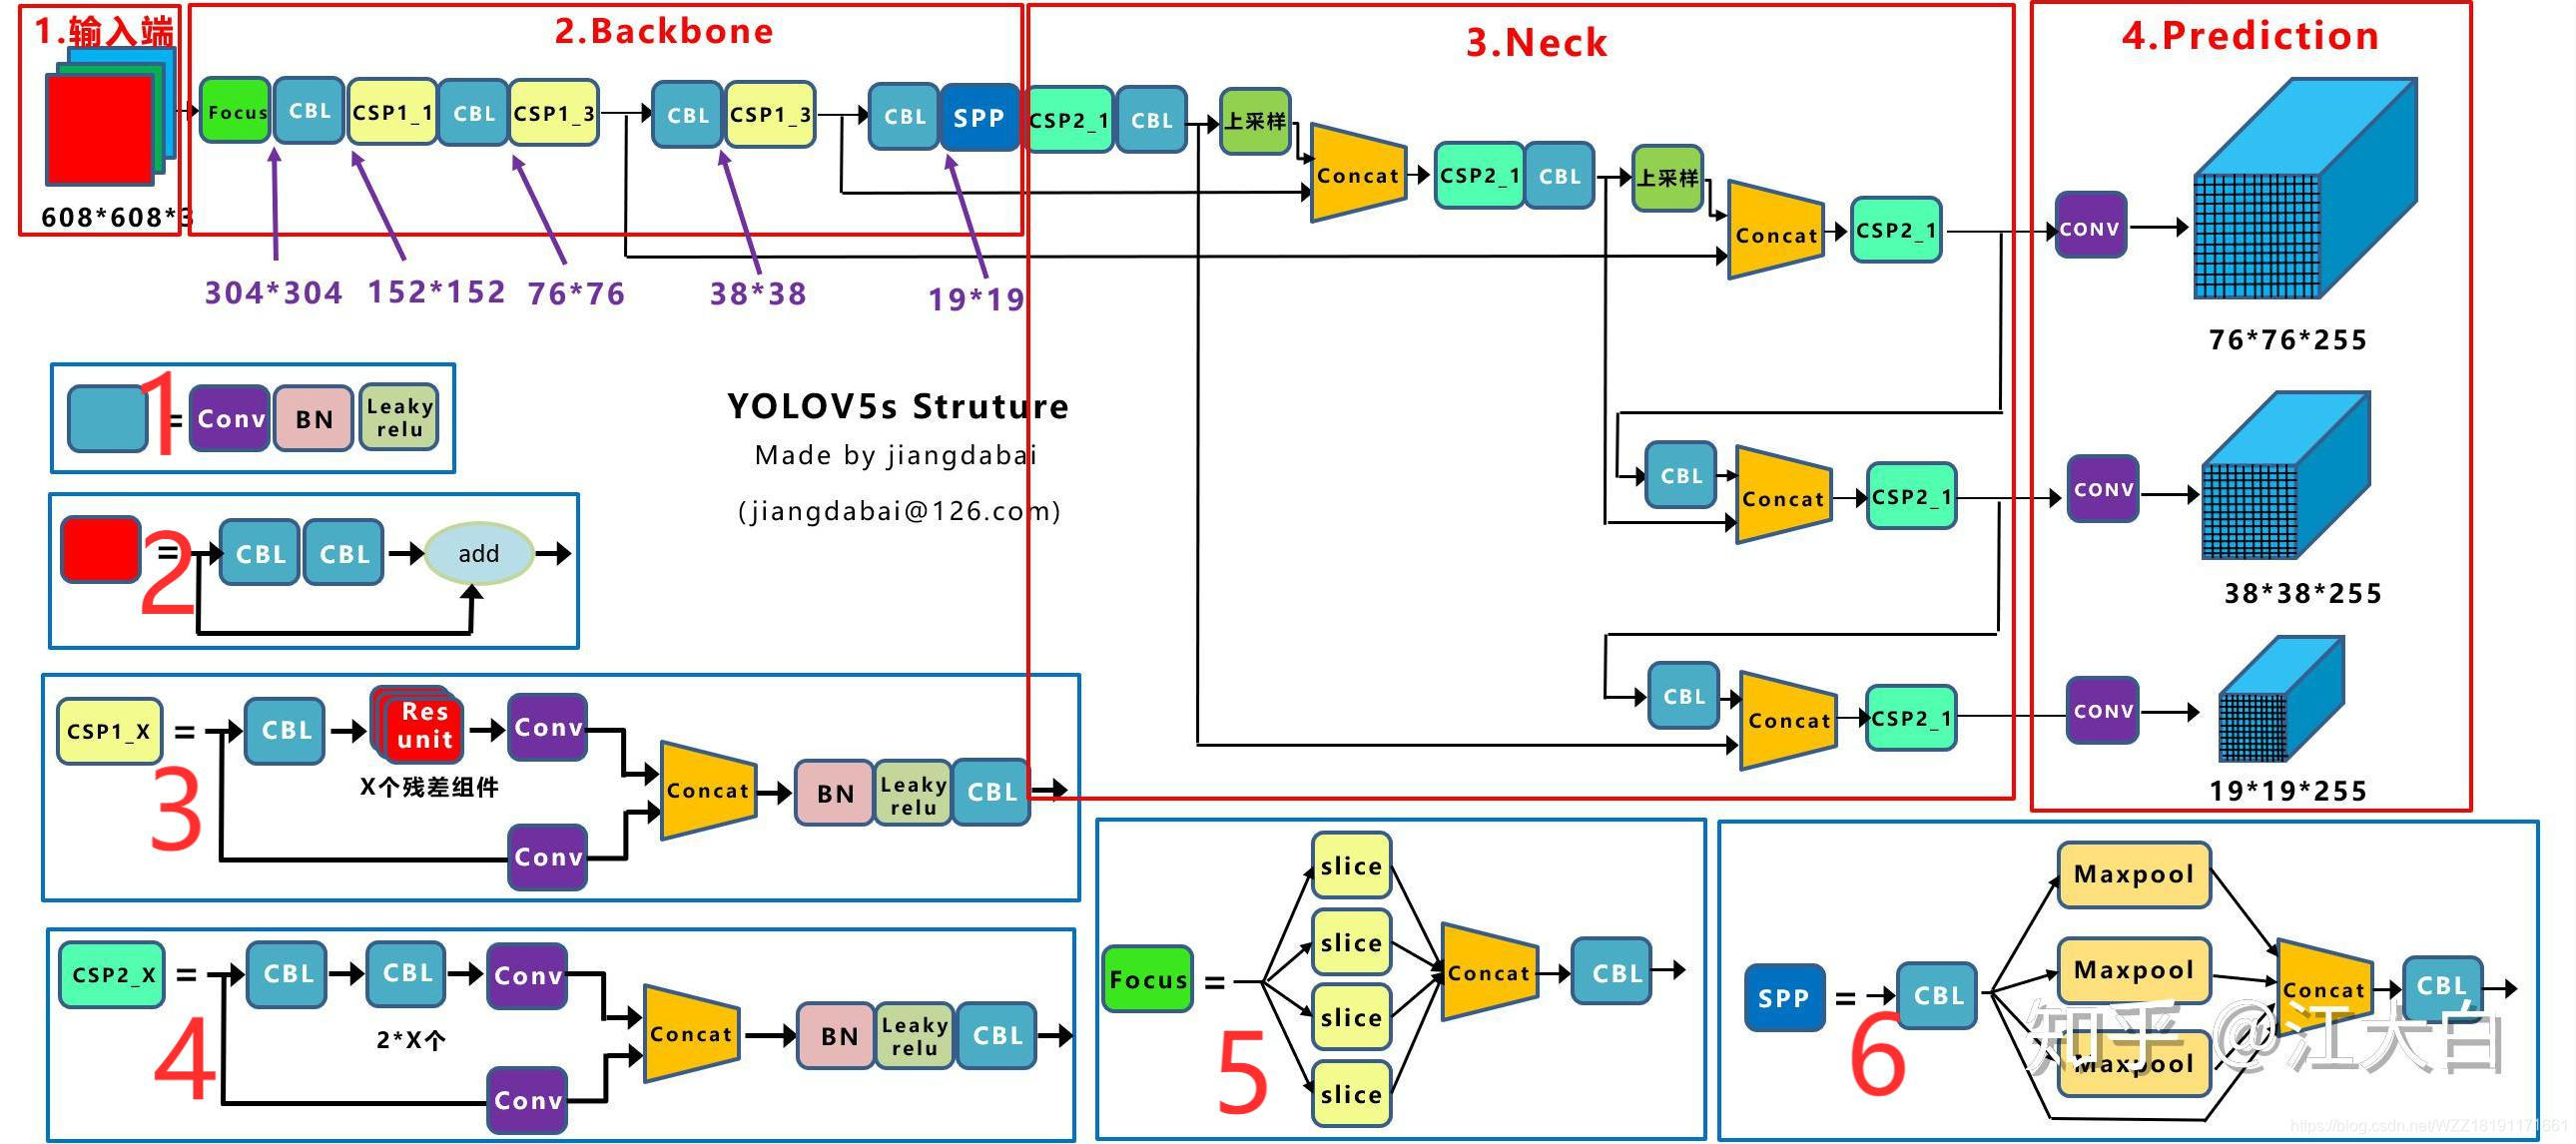
\includegraphics[width=0.8\textwidth]{images/YOLOv5.jpeg}
    \caption{YOLOv5网络架构}
    \label{fig:YOLOv5}
\end{figure}

可以通过这里了解:\url{https://github.com/THU-MIG/yolov10}

\url{https://blog.csdn.net/WZZ18191171661/article/details/113789486}

\subsection{简单了解模型部署}
如果我们已经拥有了一个训练好的模型,但是事实上这并不能草草的生搬硬套在我们实际的项目中。
一个项目通常不会是在拥有着高性能的NVIDIA显卡和高性能的CPU上运行的,通常是在一些性能较低的设备上,比如
在机器人上,代码运行在minipc,而minipc的性能和配置有限(intel旗下的nuc甚至没有GPU),因此我们需要尽量激发设备的性能,提高模型的推理速度。
这就要涉及到模型的部署。

\begin{enumerate}
    \item \textbf{CPU上的模型部署}: intel官方提供了一个完整的开源的部署工具——openvino,利用openvino提供的C++接口,可以将训练好的模型转换为openvino支持的模型,然后在CPU上运行,可以大大提高模型的推理速度。
    \item \textbf{GPU上的模型部署}: NVIDIA也提供了一个完整的开源的部署工具——tensorRT,同样也可以利用相应的API使得模型在GPU上实施推理,拥有更快的推理速度.
\end{enumerate}

\textbf{\textit{*有关模型文件类型:}}

模型文件的类型并不是单一的,不同的框架支持的是不同的文件类型。
譬如pytorch导出的模型为.pth文件,YOLO框架导出的是.pt文件。
而在openvino部署模型的时候,又需要把模型转换没xml和bin文件。
tensorrt所需的又是.engine文件。

模型文件类型的不同确实是一件麻烦的事情,因此领域内出现了一种.onnx文件,它使得不同的深度学习框架之间可以互操作。
openvino和tensorrt都支持对onnx文件的转换。有相应的API可以将onnx文件转换为自身所需要的文件类型。YOLO官方也给出了
相关的指令能够一键转换将.pt转换为.onnx文件。onnx文件就像是一个中间文件,使得不同框架之间的转换变得更加容易。

\textit{如果你有一个ONNX文件,你可以访问网站:\url{https://netron.app/}查看ONNX文件的结构,方便了解模型的结构}

\subsection{总结}
对于当今的科研工作相关人员来说,神经网络是不得不去学习的领域,同样也是一个非常重要的领域。
AI已经走进了我们的生活,无论是在自动驾驶,人脸识别,语音识别等领域,AI都有着广泛的应用。
在我们机器人的自瞄系统中,识别装甲板上的数字,识别敌方机器人,识别装甲板; 以及雷达系统,都有神经网络的身影。
感兴趣的同学可以多多学习,多多实践,祝大家学有所成。